\section[Część analityczno-teoretyczna]{Część analityczno-teoretyczna}\label{sec:theory} % 30% pracy - opis problematyki podjętego tematu w zakresie wykorzystanym w pracy i analizie
    Plazma, powszechnie nazywana czwartym stanem materii, to zbiór
    zjonizowanych cząstek oraz elektronów wykazujących jako grupa globalną
    obojętność elektryczną. Innymi słowy, od gazu plazmę odróżnia fakt, że
    cząstki są zjonizowane, więc oddziałują kolektywnie między sobą na
    odległość, ale ich pola elektryczne wzajemnie się neutralizują na długich
    dystansach.

    Plazmy występują w całym wszechświecie, od materii międzygwiezdnej po
    błyskawice.  Ich istnienie uwarunkowane jest obecnością wysokich energii,
    wystarczających do zjonizowania atomów gazu.

    Fizyka plazmy jest stosunkowo młodą nauką, której rozwój nastąpił dopiero w
    ostatnim stuleciu, zaczynając od badań Langmuira (1928), który
    eksperymentował z jonizowaniem gazów w szklanych rurach zwanych rurami
    Crookesa, służących do generowania promieniowania katodowego, czyli, jak
    wiemy obecnie, strumieni elektronów.\cite{bellan}

    Globalny wzrost zainteresowania fizyką plazmy na arenie geopolitycznej
    rozpoczął się w latach czterdziestych ubiegłego wieku, gdy uświadomiono sobie,
    że można zastosować ją do przeprowadzania kontrolowanych reakcji syntezy
    jądrowej,
    które mogą mieć zastosowania w energetyce jako następny etap rozwoju po
    reakcjach rozpadu wykorzystywanych w obecnych elektrowniach jądrowych.
    Był to jeden z elementów zimnowojennego wyścigu technologicznego między Stanami
    Zjednoczonymi a ZSRR, jak również jeden z projektów mających na celu ponowne
    nawiązanie współpracy naukowej między supermocarstwami po zakończeniu tego
    konfliktu. Obecnie trwają intensywne badania nad tym problemem, których
    dotychczasową kulminacją jest budowany we Francji tokamak ITER i planowany reaktor DEMO\@.

    Poza tym ogromnym projektem, plazmy mają szerokie zastosowania w obecnym
    przemyśle, na przykład:
    \begin{itemize}
        \itemi{} metalurgicznym --- cięcie metalu przy użyciu łuków plazmowych.
        \itemi{} elektronicznym i materiałowym --- żłobienie powierzchni urządzeń
            półprzewodnikowych, powierzchniowa obróbka materiałów, depozycja
            aktywnych jonów pod powierzchnią czyszczenie powierzchni, depozycja
            cienkich warstw związków chemicznych na powierzchniach (CVD).
        \itemi{} kosmicznym --- silniki plazmowe, interakcja z rozgrzanym powietrzem
            podczas powtórnego wchodzenia w atmosferę.
        \itemi{} użytkowym --- ekrany telewizorów, oświetlenie (świetlówki).
    \end{itemize}

    Należy też zwrócić uwagę, że ze względu na złożoność układów plazmowych
    pra-komputerowa fizyka miała ogromne problemy z merytorycznymi badaniami
    zachowania plazmy poza wybranymi, mocno uproszczonymi reżimami. Postęp w
    badaniach plazmy, jak sugeruje rozwój technologii kontrolowanej syntezy
    jądrowej, jest silnie skorelowany z
    rozwojem mocy obliczeniowej oraz algorytmów symulacyjnych.%\cite{youtube-plasma-algorithm-progress}

    \subsection{Modelowanie i symulacja plazmy}

    Modelowanie zjawisk z zakresu fizyki plazmy jest jednym z bardziej
    złożonych problemów fizyki komputerowej. Koncepcyjnie rzecz biorąc, Głównym
    powodem uniemożliwiającym zastosowanie prostych metod symulacji znanych z
    newtonowskiej dynamiki molekularnej jest mnogość oddziaływań --- każda cząstka
    oddziałuje z każdą inną nawzajem poprzez niepomijalne oddziaływania
    kulombowskie, skalujące się z odległością jak $\approx r^{-2}$. Paradoksalnie,
    na dużych odległościach oddziaływania te znoszą się, co rozumie się w plazmie
    jako \concept{kwaziobojętność} --- jednak bez uwzględnienia oddziaływań od
    wszystkich cząstek nie osiągnie się tego efektu,

    Z powodu dużej liczby cząstek w układach plazmowych, jedynym adekwatnym modelem teoretycznym
    opierającym się na fundamentalnej fizyce jest opis kinetyczny. Wielkością opisującą plazmę jest tu funkcja dystrybucji (zwana
    też funkcją rozkładu) zdefiniowana jako $f_s(\vec{x}, \vec{v}, t) d\vec{x}
    d\vec{v}$ opisująca gęstość rozkładu danej grupy cząstek $s$ plazmy w
    sześciowymiarowej przestrzeni fazowej (po trzy wymiary na położenia oraz
    prędkości). Ewolucja czasowa funkcji rozkładu dokonuje się poprzez
    rozwiązanie wariantu równania Boltzmanna zwanego równaniem Vlasova,
    które sprzęga gęstości ładunku i prądu otrzymywane z funkcji dystrybucji
    z równaniami Maxwella na ewolucję pola elektromagnetycznego.

    Dla przypadku plazmy złożonej z elektronów i jednego rodzaju jonów o ładunku $Z_i$:

    \begin{align}
    \frac{\partial f_e}{\partial t} + \vec {v}_e\cdot\nabla f_e &- e\left(\vec {E}+\vec {v_e}\times\vec {B}\right)\cdot\frac{\partial f_e}{\partial\vec {p}} = 0
    \label{eqn:vlasov-electrons}\\
    \frac{\partial f_i}{\partial t} + \vec {v}_i\cdot\nabla f_i &+ Z_i e\left(\vec {E}+\vec {v_i}\times\vec {B}\right)\cdot\frac{\partial f_i}{\partial\vec {p}} = 0
    \label{eqn:vlasov-ions}\\
    \nabla \times \vec{B} &=\mu_0 \left(\vec{j}+\epsilon_0 \frac{\partial \vec{E} }{\partial t}\right)
    \label{eqn:maxwell-B-rotation}\\
    \nabla\times\vec {E} &=-\frac{\partial\vec {B}}{\partial t}
    \label{eqn:maxwell-E-rotation}\\
    \nabla\cdot\vec {E}  &=\rho / \epsilon_0
    \label{eqn:maxwell-E-div}\\
    \nabla\cdot\vec {B}  &=0
    \label{eqn:maxwell-B-div}
    \end{align}

    Równanie Vlasova może zostać rozszerzone do równania Fokkera-Plancka uwzględniającego
    bezpośrednie kolizje międzycząsteczkowe.

    W praktyce równanie Vlasova jest trudne do rozwiązania poza trywialnymi
    przypadkami o ułatwiających problem symetriach.  Jednym z powodów tej
    trudności jest konieczność uzyskania dobrej rozdzielczości prędkości przy
    jednoczesnym zachowaniu zakresów obejmujących prędkości relatywistyczne.
    Jako równanie różniczkowe cząstkowe, równanie Vlasova jest rozwiązywane na
    dyskretnych siatkach, należy zauważyć zaś, że skalowanie
    liczby punktów na siatce tego typu jest proporcjonalne do $N_r^3 N_v^3$,
    gdzie $N_r$ to liczba punktów przestrzennych, zaś $N_v$ to liczba punktów
    na siatce prędkości. Jest to więc często niepraktyczne obliczeniowo,
    między innymi ze względu na istotne w plazmach fuzyjnych zjawisko
    ``uciekających elektronów'' o relatywistycznych prędkościach.

    W modelowaniu komputerowym plazmy stosuje się trzy główne koncepcyjne podejścia:
    \begin{enumerate}
        \itemi{} modele kinetyczne rozwiązujące bezpośrednio równania typu Vlasova
            na dyskretnych siatkach
        \itemi{} modele płynowe oparte na ciągłym opisie plazmy poprzez
            uśrednienie po dystrybucji wielkości termodynamicznych, co daje
            modele takie jak magnetohydrodynamika. Jest to wciąż układ równań
            różniczkowych cząstkowych, lecz na mniej wymiarowej siatce.
            Niestety, nie nadają się one do badań plazmy daleko od równowagi z
            powodu czynionych przy nich założeń takich jak maxwellowski rozkład
            prędkości. Znajdują za to szerokie zastosowanie w astronomii.
        \itemi{} modele dyskretne oparte na samplowaniu dystrybucji plazmy przy
            użyciu dyskretnych cząstek, pozwalające w prosty sposób uzyskać
            dobre przybliżenie faktycznego ruchu cząstek w plazmie i prądów
            generowanych tym ruchem. Pozwalają na wizualizację efektów działań
            pól, ale potrafią być mało wydajne do modelowania efektów kolektywnych.
            \todo[inline]{czy na pewno należy rozróżniać kinetyczne i dyskretne?} % TODO-WAIT
    \end{enumerate}

    Istnieje bardzo popularna klasa modeli łączących cechy kategorii pierwszej i trzeciej.
    Są to tak zwane modele Particle-in-cell.

    \subsection{Modele Particle-in-cell}

    Idea modelu \concept{particle-in-cell} (dalej nazywanego \concept{PIC}) jest wyjątkowo
    prosta i opiera się na przyspieszeniu najbardziej złożonego obliczeniowo
    kroku symulacji dynamiki molekularnej, czyli obliczania sił
    międzycząsteczkowych.  Cząstki poruszają się w ciągłej, Lagrange'owskiej
    przestrzeni.  Ich ruch wykorzystywany jest do zebrania informacji dotyczącej
    gęstości ładunku i prądu na dyskretną, Eulerowską siatkę. Na siatce rozwiązane
    są (jako równania różniczkowe cząstkowe) równania Maxwella, dzięki którym
    otrzymuje się pola elektryczne i magnetyczne, które z powrotem są przekazane do
    położeń cząstek.  Obliczeniowo, uwzględniając koszty odpowiednich interpolacji,
    pozwala to zredukować złożoność kroku obliczenia sił międzycząsteczkowych
do złożoności $O(n)$ z $O(n^2)$, gdzie $n$ jest liczbą cząstek.
    Oczywiście, jest to okupione zależnością złożoności od liczby punktów na siatce $m$, lecz jako że $m << n$,
    jest to akceptowalne i korzystne.

    \subsubsection{Pętla obliczeniowa PIC}
    Obliczeniowo algorytm particle-in-cell składa się z czterech elementów
    powtarzających się cyklicznie:
    \begin{itemize}
        \itemi{} Zbierz (\english{Gather})\\
    Depozycja ładunku oraz prądu z położeń cząstek do lokacji na dyskretnej
    siatce poprzez interpolację, co pozwala na sprawne rozwiązanie na niej
    równań Maxwella jako układu różnicowych równań cząstkowych zamiast
    obliczania skalujących się kwadratowo w liczbie cząstek oddziaływań
    kulombowskich między nimi.  W naszym elektromagnetycznym przypadku bardziej
    istotną jest depozycja prądu na siatkę, co szerzej tłumaczy następny
    fragment.
    \itemi{} Rozwiąż (\english{Solve})\\
    Sprawne rozwiązanie równań Maxwella na dyskretnej, Eulerowskiej siatce.
    Znalezienie pól elektrycznego i magnetycznego na podstawie gęstości ładunku
    i prądu na siatce.  Istnieją dwie główne szkoły rozwiązywania tych równań:
    metody globalne i lokalne. Metody globalne wykorzystują zazwyczaj równania
    dywergencyjne (prawa Gaussa)\ref{eqn:maxwell-E-div}\ref{eqn:maxwell-B-div}
    rozwiązywane iteracyjnie (metodami takimi jak Gaussa-Seidela lub gradientów
    sprzężonych)
     lub spektralnie, przy użyciu transformat Fouriera lub Hankela~\cite{fbpic}.
     Metody lokalne z kolei
    wykorzystują równania rotacyjne (prawa Ampera-Maxwella\ref{eqn:maxwell-E-rotation}
    oraz Faradaya\ref{eqn:maxwell-B-rotation}):

    Metody globalne nadają się do modeli elektrostatycznych,
    nierelatywistycznych.  Metody lokalne pozwalają na ograniczenie szybkości
    propagacji zaburzeń do prędkości światła, co przybliża metodę numeryczną do
    fizyki zachodzącej w rzeczywistym układzie tego typu.
    \itemi{} Rozprosz (\english{Scatter}) \\
    Interpolacja pól z siatki do lokacji cząstek, co pozwala określić siły
    elektromagnetyczne działające na cząstki.  Należy przy tym zauważyć, że
    jako że interpolacja sił wymaga jedynie lokalnej informacji co do pól
    elektromagnetycznych w okolicy cząstki, ta część sprawia, że
    algorytmy Particle-in-cell doskonale nadają się do zrównoleglenia (problem
    jest w bardzo dobrym przybliżeniu ``trywialnie paralelizowalny''). Z tego
    powodu algorytmy Particle-in-cell nadają się doskonale do wykorzystania
    rosnącej mocy kart graficznych i architektur GPGPU\@.
    \itemi{} Porusz (\english{Push}) \\
    iteracja równań ruchu cząstek
    \begin{equation}
        d \vec{p}/dt = \vec{F} = q (\vec{E} + \vec{v} \times \vec{B})
        \label{eq-of-motion}
    \end{equation}
    na podstawie ich prędkości (aktualizacja położeń) oraz działających na nie
    sił elektromagnetycznych (aktualizacja prędkości). Należy zauważyć, że
    modele PIC nie modelują bezpośrednich kolizji między cząstkami. Kolizje
    mogą jednak zostać dodane niebezpośrednio, na przykład poprzez metody Monte
    Carlo.

    Jako że każda cząstka, zakładając znane pola elektromagnetyczne w jej
    położeniu, porusza się niezależnie, jest to kolejny fragment doskonale
    nadający się do zrównoleglenia.
    \end{itemize}
    \subsubsection{Makrocząstki}
    Należy zauważyć, że obecnie nie jest jeszcze możliwe dokładne odwzorowanie
    dynamiki układów plazmowych w sensie interakcji między poszczególnymi
    cząstkami ze względu na liczbę cząstek rzędu liczby Avogadro $\approx
    10^{23}$.  W tym kontekście bardzo korzystnym jest fakt, że wszystkie
    istotne wielkości zależą nie od ładunku ani masy, ale od stosunku $q/m$. W
    praktyce stosuje się więc \emph{makrocząstki}, obdarzone ładunkiem i masą
    będące wielokrotnościami tych wielkości dla cząstek występujących w naturze
    (jak jony i elektrony), pozwalając jednocześnie zachować koncentracje cząstek,
    gęstości ładunku i prądu zbliżone do rzeczywistych.

    Makrocząstki posiadają też kształt, który wyraża się w symulacji poprzez
    interpolację wielkości fizycznych znanych na siatce Eulera do położeń
    cząstek i odwrotnie. Matematycznie jest to opisane poprzez funkcję kształtu.
    Najprostszą jednowymiarową funkcją kształtu, oznaczaną $S_0$, jest funkcja
    ``cylindrowa'', która oznacza jednorodny rozkład gęstości cząstki w zakresie
    szerokości równym długości jednej komórki.
    
    Inne funkcje kształtu tworzy się poprzez kolejne sploty funkcji podstawowej,
    co obrazuje rysunek\ref{fig:shapefunctions}. Funkcja $S_1$ (trójkątna,
    skupiona na środku) jest tradycyjną funkcją kształtu wykorzystywaną
    historycznie w większości zastosowań modelu PIC\@.


    \begin{figure}[h!]
      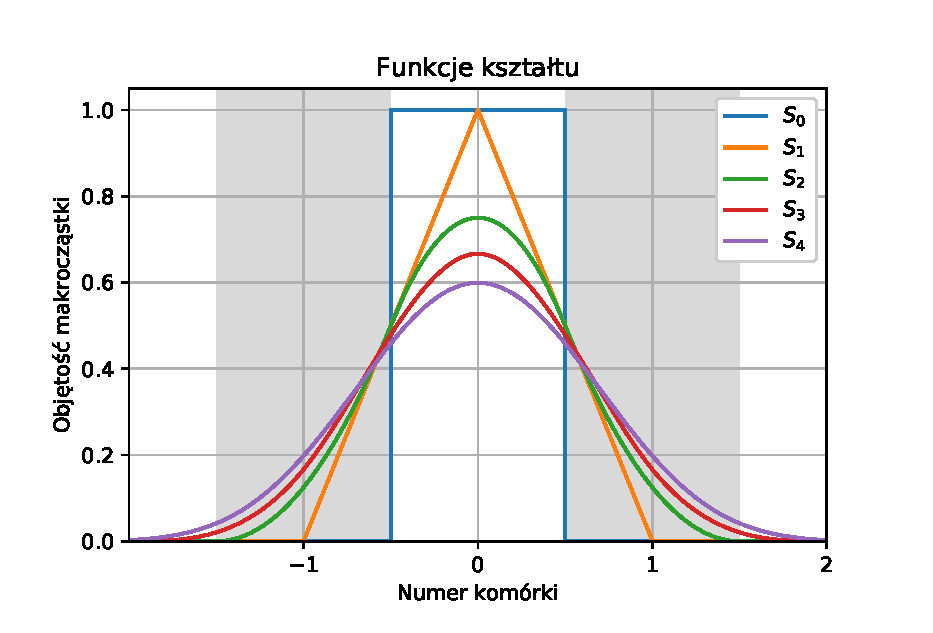
\includegraphics{Images/shapefunctions}
      \caption{Typowe funkcje kształtu dla makrocząstki\label{fig:shapefunctions}} 
    \end{figure}

    W symulacjach elektromagnetycznych zazwyczaj stosuje się
    gęstości cząstek (rzeczywistych) rzędu jednej dziesiątej bądź setnej
    gęstości krytycznej plazmy $n_c$ (wyrażaną wzorem~\ref{eqn:critical-density}),
    która oznacza taką koncentrację
    elektronów, przy której fala laserowa zaczyna być tłumiona zamiast być
    przepuszczaną przez plazmę.\cite{chen}

    \begin{equation}
        n_c = m_e \varepsilon_0 {(\frac{2 \pi c}{e \lambda})}^2
        \label{eqn:critical-density}
    \end{equation}
    gdzie $m_e$ to masa spoczynkowa elektronu, $\varepsilon_0$ to przenikalność
    elektryczna próżni, $c$ to prędkość światła w
    próżni, $e$ to ładunek elementarny, zaś $\lambda$ to długość fali.

    Gęstość takiej makrocząstki, oznaczana $n_{pic}$, oznacza innymi słowy
    liczbę rzeczywistych cząstek, jakie reprezentuje sobą jedna makrocząstka.

    \subsection{Problem testowy}\label{seq:lasershield}

    Głównym problemem testowym, jakiego używamy do przetestowania dokładności i
    wydajności działania algorytmu jest interakcja impulsu laserowego z tarczą
    składającą się ze zjonizowanego wodoru i elektronów.

    Układ ten modelowany jest jako jednowymiarowy. Jest to tak zwany w
    literaturze model 1D-3D.  O ile położenia cząstek są jednowymiarowe ze
    względu na znaczną symetrię cylindryczną układu, cząstki mają prędkości w
    pełnych trzech wymiarach. Jest to konieczne ze względu na oddziaływania
    cząstek z polem elektromagnetycznym propagującym się wzdłuż osi układu
    i możliwość dowolnego dobrania kierunku polaryzacji promieniowania
    laserowego w symulacji.

    Układ ten jest silnie zbliżony do rzeczywistych eksperymentów prowadzonych
    w Instytucie Fizyki Plazmy i Laserowej Mikrosyntezy.  \todo[inline]{Tu bym
    chciał prosić o weryfikację.} % TODO-WAIT

